\section{Entanglement in front of a thermal shield}\label{sec:5:thermal-entanglement}
The entanglement generation between the two particles depends heavily on the variation of the separation between the shield and the particles, as has been seen in \cref{cha:entanglement-generation}.
The vibrating shield can be interpreted as varying the separation and angle of the cat-state in front of the plate - visualized in \cref{fig:5:vibrating-translation-to-variations}.
\begin{figure}[!htbp]
  \centering
  \def\svgwidth{\textwidth}
  \input{./../figures/plate-vibration.pdf_tex}
  \caption{For a large $r_s \gg R$ and locally flat shield, the thermal vibrations with amplitude $z$ can be interpreted as a static shield where the particle $A$ (shown in the figure) is placed at $L+\Delta L$ at angle $\theta$ and particle $B$ is places at $L-\Delta L$ with angle $-\theta$ where both variations depend on the amplitude. At low vibrational frequencies $1/\omega \approx t_\mathrm{max}$ the amplitude can be assumed to be static during a experimental run and for each measurement thermally distributed around $\mean{z}=0$ with $\Delta z$ given by eq. \eqref{eq:5:amplitude-variance}.}
  \label{fig:5:vibrating-translation-to-variations}
\end{figure}
This is only a good approximation for shields larger than the particles radius $r_s \gg R$ and low vibrating frequencies $1/\omega \approx t_\mathrm{max}$ and can therefore be used well to describe the highly disturbing first few modes on a large shield.
Furthermore, this interpretation is possible because as shown in \cref{sec:3:imperfect-plates}, the Casimir interaction between a sphere and a tilted plane does not differ from the interaction between a flat plane.
Contrary to the problem considered in \cref{cha:entanglement-generation}, here only the thermal amplitude $z_{kl}$ is a independent random variable distributed around $\mean{z_{kl}} = 0$ with standard deviation $\Delta z_{kl}$ given by eq. \eqref{eq:5:amplitude-variance}. 
Both, the variations in the particle-shield separation $\Delta L$ as well as in the angle $\theta$ are correlated to the amplitude $z$.
For a large shield, this can be understood as
\begin{equation}
  \theta = \arctan(z \abs{\nabla u}) \approx z \abs{\nabla u} \quad \text{and} \quad \Delta L = z \abs{u}
\end{equation}
where $\nabla u$ is the gradient of the shape of the vibrational mode.
Performing similar calculations as done before in \cref{cha:entanglement-generation}, the averaged density matrix $\mean{\rho}$ dependent on $\Delta z_{kl}$ can be calculated and is given in \cref{apx:density-matrix-vibrating-plate}.
The entanglement quantified by the logarithmic negativity \cite{Plenio_2005} introduced in \cref{sec:2:entanglement-measures} dependent on the temperature $T$ and on the particle-shield separation $L$ is shown in \cref{fig:5:entanglement-temperature}.
\begin{figure}[!htbp]
  \centering
  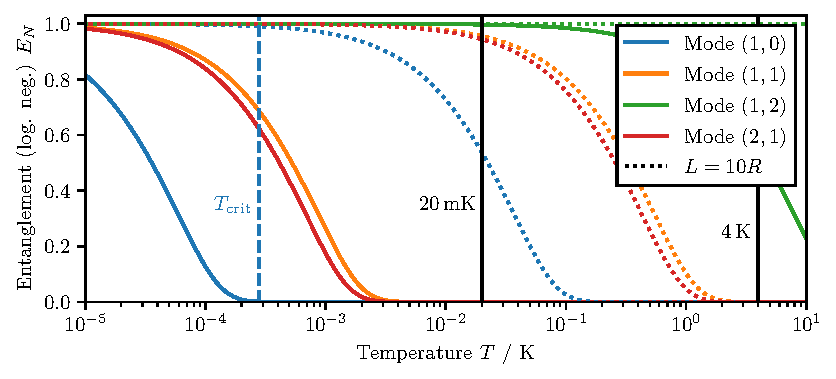
\includegraphics[width=\textwidth]{./../figures/vibrations/log-neg-shield-vibrations-T.pdf}
  \caption{Entanglement between the particles (parallel orientation) in front of a thermal shield at different temperature $T$ for selected modes. At a temperature $T_\mathrm{crit,\,kl}$, all entanglement is lost if the mode $(k,l)$ is present. This critical point shifts with higher separation distance $T_\mathrm{crit}\propto L^4$}
  \label{fig:5:entanglement-temperature}
\end{figure}
At reasonable temperatures, entanglement in the presence the mode $(1,0)$ is in theory only observable for large separations.
In fact, the dependence of the critical temperature $T_\mathrm{crit}$ on the separation $L$ is known as for large separation in the LSL the following is expected:
\begin{equation}
  T_\mathrm{crit} \sim (\Delta z_\mathrm{crit})^2 \sim \left(\frac{L^5}{t_\mathrm{max}} \right)^2 \sim L^4 .
\end{equation}
The required large separations are surprising considering that the thermal amplitudes $\Delta z_{1,0} \approx 9 \times 10^{-11}\si{m}$ at $20\si{mK}$ which is comparable with the previously calculated values for $\Delta L_\mathrm{crit}$ in \cref{cha:entanglement-generation}.
Interestingly this result does not change for different shield radii - at least as long as the condition $r_s \ll R$ is fulfilled and the shield shape can locally be linearized.
This is because the gradient $\abs{\nabla u} \propto 1/r_s$ which perfectly cancels with the dependence on $z \propto r_s$ leaving $\theta$ independent of $r_s$. 
If the cat-state orientation is now chosen parallel to the shield, the dependence on $\Delta L$ is irrelevant leaving the final resulting entanglement independent of $r_s$.
However, as seen in \cref{fig:5:entanglement-temperature}, the mode number $(k,l)$ has a huge effect on the entanglement generation. As stated before, higher modes correspond to a higher vibrational frequency and thus smaller amplitudes $\Delta z$.
Asymptotically, therefore a scaling of $T_\mathrm{crit}$ in the order of $\mathcal{O}(k^2 + l^2)$ is expected.
\begin{figure}[!htbp]
  \centering
  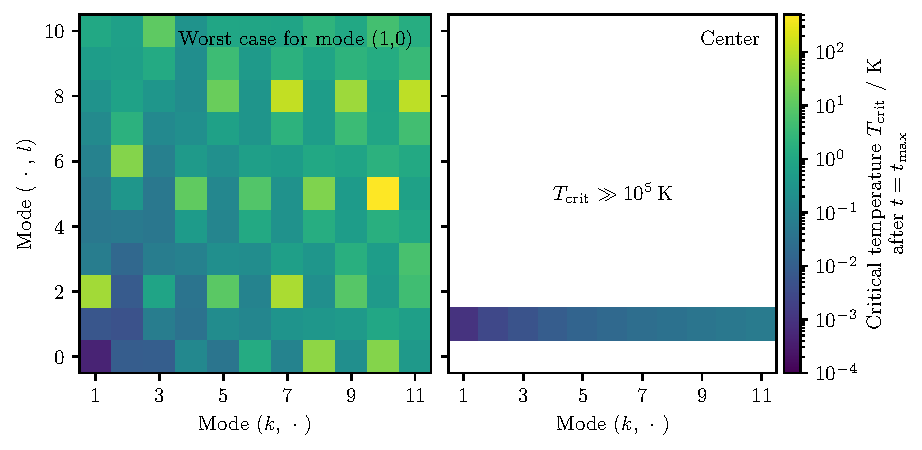
\includegraphics[width=\textwidth]{./../figures/vibrations/T-crit-modes.pdf}
  \caption{Critical temperature $T_\mathrm{crit}$, at which no entanglement is measurable anymore for different modes at a separation of $L = 2R = 2\si{\mu m}$.}
  \label{fig:5:T-crit-modes}
\end{figure}
It becomes evident, that only the first couple of modes are actually relevant as all others do not destroy entanglement up to temperatures much higher than necessary.



\subsection{Analytic dynamics}
Surprisingly the influence of the thermal shield on entanglement generation can be calculated analytically.
% \begin{align}\label{eq:5:hamiltonian}
% \begin{split}
%   \op{H} = \sum_{\substack{m\in\{(k,l)\}\\ k \geq 1,\ l \geq 0}} \biggl\{ & \hbar \omega_m \left(\op{a}^\dagger_m \op{a}_m + \frac{1}{2}\right) \\
%   &+ \left(g^1_\mathrm{A,m,Cas} + g^1_\mathrm{B,m,Cas}\right)(\op{a}_m + \op{a}^\dagger_m) \ketbra{\psi^1_A \psi^1_B} \\
%   &+ \left(g^1_\mathrm{A,m,Cas} + g^2_\mathrm{B,m,Cas}\right)(\op{a}_m + \op{a}^\dagger_m)\ketbra{\psi^1_A \psi^2_B} \\
%   &+ \left(g^2_\mathrm{A,m,Cas} + g^1_\mathrm{B,m,Cas}\right)(\op{a}_m + \op{a}^\dagger_m)\ketbra{\psi^2_A \psi^1_B} \\
%   &+ \left(g^2_\mathrm{A,m,Cas} + g^2_\mathrm{B,m,Cas}\right)(\op{a}_m + \op{a}^\dagger_m)\ketbra{\psi^2_A \psi^2_B}\biggr\} \\
%   + g^{1,1}_\mathrm{Grav}&\ketbra{\psi^2_A \psi^2_B} + g^{1,2}_\mathrm{Grav}\ketbra{\psi^2_A \psi^2_B} \\
%   + g^{2,1}_\mathrm{Grav}&\ketbra{\psi^2_A \psi^2_B} + g^{2,2}_\mathrm{Grav}\ketbra{\psi^2_A \psi^2_B}
% \end{split}
% \end{align}
\begin{align}\label{eq:5:hamiltonian}
  \begin{split}
    \op{H} = \sum_{\substack{m\in\{(k,l)\}\\ k \geq 1,\ l \geq 0}} \biggl\{ & \hbar \omega_m \left(\op{a}^\dagger_m \op{a}_m + \frac{1}{2}\right) \\
    &+ g^1_\mathrm{A,m,Cas}(\op{a}_m + \op{a}^\dagger_m) \left( \ketbra{\psi^1_A} \otimes \identity \right)
     + g^2_\mathrm{A,m,Cas}(\op{a}_m + \op{a}^\dagger_m) \left( \ketbra{\psi^2_A} \otimes \identity \right) \\
    &+ g^1_\mathrm{B,m,Cas}(\op{a}_m + \op{a}^\dagger_m) \left( \identity \otimes \ketbra{\psi^1_B} \right)
     + g^2_\mathrm{B,m,Cas}(\op{a}_m + \op{a}^\dagger_m) \left( \identity \otimes \ketbra{\psi^2_B} \right)\biggr\} \\
    + g^{1,1}_\mathrm{Grav}&\ketbra{\psi^1_A \psi^1_B} + g^{1,2}_\mathrm{Grav}\ketbra{\psi^1_A \psi^2_B} \\
    + g^{2,1}_\mathrm{Grav}&\ketbra{\psi^2_A \psi^1_B} + g^{2,2}_\mathrm{Grav}\ketbra{\psi^2_A \psi^2_B}
  \end{split}
\end{align}
where $g^{ij}_\mathrm{Grav}$ is the gravitational coupling between the states $\ket{\psi^i_A}$ and $\ket{\psi^j_B}$ which is similar like previously, as it is independent of the shield movement at all.
The gravitational coupling between the shield and the particles have been neglected here, as this coupling is by a factor $10^{7}$ times weaker than the Casimir interaction.
This interaction between state $\ket{\psi_{A(B)}^i}$ and the shield is denoted by $\tilde{g}^i_\mathrm{A(B),\,m,\,Cas}$. These couplings are dependent on the amplitude $\op{z}_{m} = \sqrt{\hbar/2\tilde{m}\omega_m} (\op{a}_m + \op{a}^\dagger_m)$ and the shape $u_{m}(r_{A(B)})$ of the vibrational mode $m\in\{(k,l)\}$ at the position $r_{A(B),i}$ of the cat state:
\begin{equation}
  \tilde{g}^i_\mathrm{A(B),\,m,\,Cas} = \frac{\hbar c \pi^3}{720} \left(\frac{\varepsilon_r - 1}{\varepsilon_r + 1}\right)\varphi(\varepsilon_r) \frac{R}{(\mathscr{L} + \op{z}_m u_m(r))^2} \approx g_\mathrm{PFA} \left(\frac{1}{\mathscr{L}^2} + \frac{2 \op{z}_m u_m(r_{A(B),i})}{\mathscr{L}^3}\right) .
\end{equation}
Ignoring the first term in the expansion, which just produces a global phase in the evolved system, the couplings $g_\mathrm{Cas}$ appearing in eq. \eqref{eq:5:hamiltonian} are finally given by
\begin{equation}
  g^i_\mathrm{A(B),\,m,\,Cas} = g_\mathrm{PFA} \frac{2u_m(r_{A(B),i})}{\mathscr{L}^3} \sqrt{\frac{\hbar}{2 \tilde{m} \omega_m}} .
\end{equation}
It is possible to analytically calculate the time evolution of a system consisting of the initial state $\rho_\mathrm{system}$ (given by eq. \eqref{eq:2:initial-state}) combined with the infinite vibrational modes $\rho_\mathrm{th}$ of the thermal shield
\begin{equation}
  \rho_0 = \bigotimes_{m\in\{(k,l)\}} \left(\rho_\mathrm{th,\,m}\right) \otimes \rho_\mathrm{system} .
\end{equation}
These thermal states can be expanded into coherent states $\ket{\alpha} = \op{D}(\alpha)\ket{0}$ as \cite{Steiner_2024}
\begin{equation}
  \rho_\mathrm{th,m} = \frac{1}{Z} \sum_{n=1}^{\infty} e^{-\beta \hbar \omega_m (n + 1/2)} \ketbra{n} = \int \dd \alpha^2 \frac{1}{\pi \bar{n}} e^{-\frac{\abs{\alpha}^2}{\bar{n}}} \ketbra{\alpha}
\end{equation}
where $\bar{n}$ is the average occupation number. The time evolution of the particle-system $\rho_\mathrm{system}(t) = \tr_{th}\left\{\rho(t)\right\}$ can be calculated by tracing out all states corresponding to the thermal shield.

\begin{equation}
  \gamma_{ij} = \sum_{m\in{(k,l)}} \frac{4}{\hbar^2\omega_m^2} \abs{(g_A + g_B) - (g_A + g_B)}^2 \sin^2\left(\frac{\omega_m t}{2}\right) \left[\bar{n} + \frac{1}{2}\right]
\end{equation}
\begin{equation}
  \varphi_{ij} = \sum_{m\in{(k,l)}} \frac{i}{\hbar} \left( g_\mathrm{Grav} - g_\mathrm{Grav} \right) t + \frac{i}{\hbar^2\omega_m^2}\left[(g_A + g_B)^2 - (g_A + g_B)^2\right]
\end{equation}

\begin{figure}[!htbp]
  \centering
  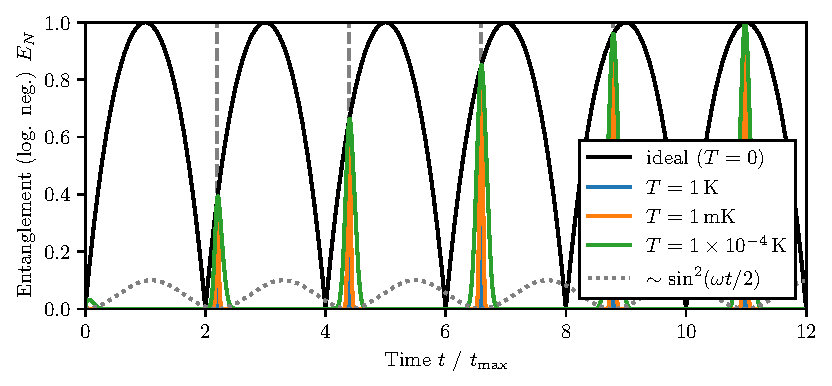
\includegraphics[width=\textwidth]{./../figures/vibrations/entanglement-hamiltonian.pdf}
  \caption{Entanglement dynamics in front of a thermal shield in mode $(1,0)$ at different temperatures. Only at specific times $2\pi k / \omega_{1,0},\ k\in\mathbb{N}$, entanglement is observable. This behavior is expected and aligns with the findings in Ref. \cite{Pedernales_2022}.}
\end{figure}

\begin{figure}[!htbp]
  \centering
  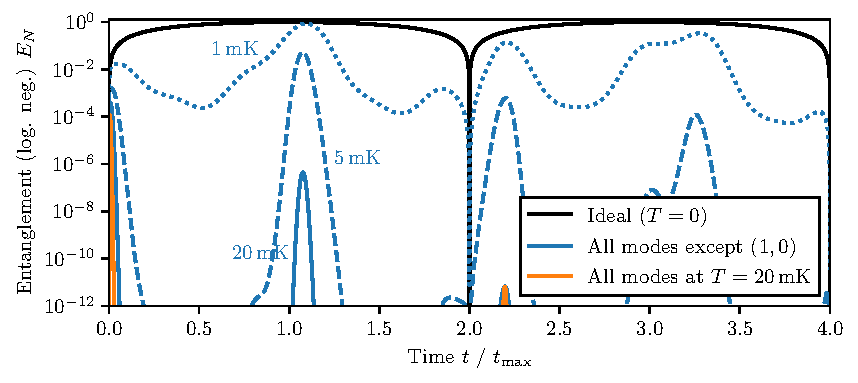
\includegraphics[width=\textwidth]{./../figures/vibrations/entanglement-multiple-modes.pdf}
  \caption{Entanglement dynamics in front of a thermal shield. In orange, the first 50 modes have been used in the numeric calculation. The effect of all remaining modes is around $1.7 \times 10^{-11}\,\%$. In blue, all modes except the first mode $(1,0)$ have been considered at different temperatures ranging vom $1\si{mK}$ up to $20\si{mK}$. The particle-shield separation is fixed at $L = 2R = 20\si{\mu m}$.}
\end{figure}

\begin{figure}[!htbp]
  \centering
  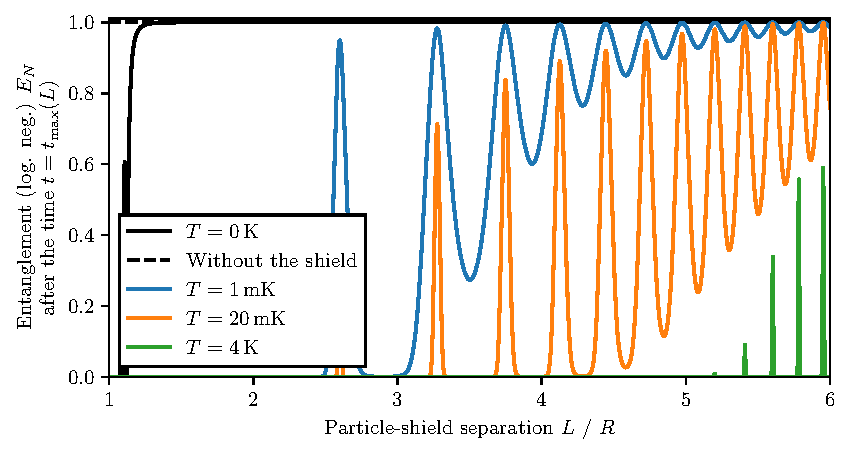
\includegraphics[width=\textwidth]{./../figures/vibrations/all-modes-entanglement-L-t-max.pdf}
  \caption{All modes, Entanglement at t-max(L)}
\end{figure}

- Without gravity

- Time omega/2pi is only dependent on the shield size and so on but tmax is dependent on the distance -> confusing

- Only entanglement at very specific times -> Modes never align

- No gca() so no repeating pattern

- Larger separation required for more measurable entanglement

- Explain why in the figure T=0 is not the same as without the shield


\subsection{Small shields}
For very small shields in the size of the particles $r_s \sim R + \Delta x / 2$, the above considerations do not hold as they required a local linearization of the vibrational mode.
A small shield only can block the direct Casimir interactions between the particles $A$ and $B$ and therefore only be used if no other forms of electromagnetic interactions between the particles such as Coulomb coupling is present.
The shield vibrations have a direct effect on the casimir interactions between the particle and the plate as the plate can no longer be approximated as locally flat or slightly tilted.
As seen in \cref{sec:3:imperfect-plates} deformations in the form of e.g. the first vibrational mode have a large effect on the resulting Casimir potential in the proximity-force-approximation resulting in a interaction roughly equivalent between a sphere and a plate at a separation of $\mathscr{L} \pm \Delta z$. 
